\documentclass[12pt]{article}

\setlength{\parindent}{0pt}
\setcounter{secnumdepth}{3}
\usepackage[margin=1in]{geometry}

% packages
\usepackage{amsmath, amsfonts, amsthm, amssymb}
\usepackage{graphicx, float}
\usepackage{mathtools}
\usepackage{titlesec}
\usepackage{interval}
\usepackage{hyperref}
\usepackage{siunitx}
\usepackage{titling}
\usepackage{vwcol}
\usepackage{setspace}
\usepackage{empheq}
\usepackage{cancel}
\usepackage{esdiff}
\usepackage{multicol}
\usepackage{mdframed}
\usepackage{esdiff}
\usepackage{tikzsymbols}
\usepackage{multicol}
\usepackage{tikz}
\usepackage{varwidth}
\usepackage{pgfplots}
\usepackage{fancyhdr}
\usepackage{enumitem}
\usepackage{tcolorbox}

\intervalconfig {
	soft open fences
}

% header
\pagestyle{fancy}
\fancyhf{}
\lhead{Ethan Fan}
\rhead{PCH}
\cfoot{\thepage}

% section format
\titleformat{\section}
  {\bfseries}
  {}
  {0em}
  {}
\titlespacing*{\section}{0pt}{0pt}{0.3em}

\titleformat{\subsection}[runin]
  {\bfseries}
  {}
  {0em}
  {}
\titlespacing*{\subsection}{0pt}{0pt}{0em}

\titleformat{\subsubsection}[runin]
  {\itshape}
  {(\roman{subsubsection})}
  {0em}
  {}

% commands
\newcommand{\alignedintertext}[1]{%
  \noalign{%
    \vskip\belowdisplayshortskip
    \vtop{\hsize=\linewidth#1\par
    \expandafter}%
    \expandafter\prevdepth\the\prevdepth
  }%
}

\newcommand*{\paren}[1]{\ensuremath\left(#1\right)}
\newcommand*{\limit}[2][x]{\ensuremath{\displaystyle\lim_{#1\to#2}}}
\newcommand*{\Limit}[3][x]{\ensuremath{\displaystyle\lim_{#1\to#2}\left[#3\right]}}
\newcommand*{\deriv}[1][x]{\ensuremath{\dfrac{\mathrm{d}}{\mathrm{d}#1}}}
\newcommand*{\Deriv}[2][x]{\ensuremath{\dfrac{\mathrm{d}}{\mathrm{d}#1}\left[#2\right]}}
\newcommand{\dydx}{\frac{dy}{dx}}
\newcommand*{\iinteg}[2][x]{\ensuremath{\displaystyle\int #2\;\mathrm{d}#1}}
\newcommand*{\dinteg}[4][x]{\ensuremath{\displaystyle\int_{#2}^{#3}#4\;\mathrm{d}#1}}
\newcommand*{\abs}[1]{\ensuremath{\left|#1\right|}}
\newcommand*{\eps}{\varepsilon}
\newcommand*{\real}{\ensuremath\mathbb{R}}
\newcommand*{\integer}{\ensuremath\mathbb{Z}}
\newcommand*{\posint}{\ensuremath\mathbb{Z^+}}
\newcommand*{\cbrt}[1]{\ensuremath{\sqrt[3]{#1}}}
\newcommand*{\lheqzero}{\ensuremath{\underset{\text{L'H}}{\overset{\left[\frac00\right]}{=}}}}
\newcommand*{\lheqinfty}{\ensuremath{\underset{\text{L'H}}{\overset{\left[\frac{\infty}{\infty}\right]}{=}}}}
\newcommand{\tor}{\text{ or }}
\newcommand{\floor}[1]{\lfloor #1 \rfloor}

\newcommand{\vem}{\vspace{0.5em}}
\newcommand{\example}[1]{\section{Example #1}}
\newcommand{\problem}[1]{\section{Problem #1}}
\newcommand{\subproblem}[1]{\subsection{(#1)} \,}

\DeclareMathOperator{\dne}{DNE}
\DeclareMathOperator{\sgn}{sgn}

\newcommand{\definition}[1]{\begin{tcolorbox}[colback=red!5!white,colframe=red!75!black,parbox=false] #1 \end{tcolorbox}}

\newcommand{\theorem}[2]{\begin{tcolorbox}[title={#1},colback=blue!5!white,colframe=blue!75!black,parbox=false] #2 \end{tcolorbox}}

\allowdisplaybreaks
% \postdisplaypenalty=100000

% document
\begin{document}

\vspace*{0cm}

% opening
\begin{center}
    {\Large \bfseries Problem Set 71} \\[0.5cm]
    {\large Collection of Problems on Monotonicity and Extrema} \\[0.35cm]
    {\normalsize May 1, 2026}
\end{center}

% problems

\problem{1}
Find the range of the following function using I/D test: \vem

\subproblem{b} $f(x)=\dfrac{1}{\pi}(\arcsin x+\arctan x)+\dfrac{x+1}{x^2+2x+5}$
\begin{gather*}
    x\in [-1,1]\\
    f'(x)=\frac{1}{\pi}(\frac{1}{\sqrt{1-x^2}}+\frac{1}{1+x^2})+\frac{-(x+3)(x-1)}{(x^2+2x+5)^2}\\
    f'(x)>0, x\in (-1,1)
\end{gather*}
As $f'(x)>0$ on $(-1,1)$, $f(x)$ monotonically increases on this interval.
\begin{gather*}
    f(-1)=\frac{1}{\pi}(-\frac{\pi}{2}-\frac{\pi}{4})+0=-\frac{3}{4}\\
    f(1)=\frac{1}{\pi}(\frac{\pi}{2}+\frac{\pi}{4})+\frac{2}{8}=1\\
    \boxed{f(x)\in [-\frac{3}{4},1]}
\end{gather*}

\problem{2}
Find the number of roots of the function using I/D test: $f(x)=\dfrac{1}{(x+1)^3}-3x+\sin x$.
\begin{gather*}
    f'(x)=-\frac{3}{(x+1)^4}-3+\cos x\\
    f'(x)<0, \quad x\in (-\infty,-1) \cup (-1,\infty)\\
    f(-1^-)\to -\infty, f(-1^+)\to \infty\\
    \boxed{2  \text{ roots}}
\end{gather*}

\problem{3}
Use I/D test to prove that:\vem

\subproblem{a}
$\ln (1+x)<x$ for $x>0$
\begin{gather*}
    f(x)=x-\ln(1+x)\\
    f(0)=0-\ln 1=0\\
    f'(x)=1-\frac{1}{1+x} \implies f'(x)>0\\
\end{gather*}
As $f'(x)>0$ on $\mathbb{R}$, $f(x)$ monotonically increases on $\mathbb{R}$.
\[
\boxed{x>\ln (1+x)}
\]

\subproblem{b}
$\sin x <x$ and hence $\cos (\sin x)>\sin(\cos x)$ for $0<x<\dfrac{\pi}{2}$
\begin{gather*}
    f(x)=x-\sin x\\
    f'(x)=1-\cos x\\
    x\in (0,\frac{\pi}{2}) \implies f'(x)>0
\end{gather*}
As $f'(x)>0$ on $(0,\dfrac{\pi}{2})$, $f(x)$ monotonically increases on this interval.
\begin{gather*}
    \boxed{x>\sin x}\\
    \cos x>\sin (\cos x)\\
    \sin(\frac{\pi}{2}-x)>\sin (\cos x)\\
    \sin(\frac{\pi}{2}-\sin x)>\sin(\frac{\pi}{2}-x)>\sin (\cos x)\\
    \boxed{\cos (\sin x)>\sin (\cos x)}
\end{gather*}

\problem{4}
\subproblem{a}
Find the relative maximum and/or minimum (if any) of the function $f(x)=(\dfrac{1}{x})^x$.
\begin{gather*}
    y=(\dfrac{1}{x})^x\\
    \ln y=x\ln \frac{1}{x}\\
    \frac{y'}{y}=\ln \frac{1}{x}+x\cdot x\cdot -\frac{1}{x^2}\\
    f'(x)=(\dfrac{1}{x})^x(\ln \frac{1}{x}-1)\\
    f'(x)=0 \implies \ln \frac{1}{x}=1\\
    \boxed{x=\frac{1}{e}}
\end{gather*}
As $f'(x)$ changes from positive to negative at $x=\dfrac{1}{e}$, $f(x)$ has a relative maximum at $x=\dfrac{1}{e}$.

\subproblem{b}
Sketch the graph of $f(x)$.
\begin{gather*}
    \lim_{x\to 0^+}f(x)=1\\
    \lim_{x\to \infty}f(x)=0
\end{gather*}
\begin{figure}[H]
    \centering
    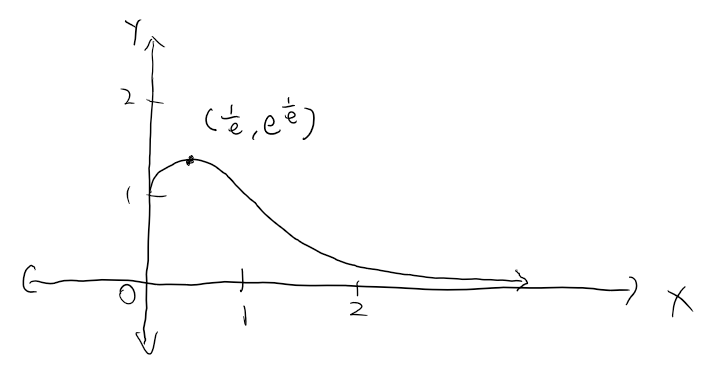
\includegraphics[width=0.5\linewidth]{q4.png}
\end{figure}

\subproblem{c}
Find the range of $f(x)$.
\begin{gather*}
    x\in (0,\infty)\\
    f(\frac{1}{e})=e^\frac{1}{e}\\
    \lim_{x\to \infty}f(x)=0\\
    \boxed{f(x)\in (0,e^\frac{1}{e}]}
\end{gather*}

\subproblem{d}
Determine which is bigger, $(\dfrac{1}{\pi})^\frac{1}{e}$ or $(\dfrac{1}{e})^\frac{1}{\pi}$?
\begin{gather*}
    \text{Define } f(x)=(\frac{1}{x})^{\frac{1}{\pi+e-x}}\\
    \ln f(x)=\frac{\ln \frac{1}{x}}{\pi+e-x}\\
    \frac{f'(x)}{f(x)}=\frac{-\frac{\pi+e-x}{x}+\ln \frac{1}{x}}{(\pi+e-x)^2}\\
    f'(x)=(\frac{1}{x})^{\frac{1}{\pi+e-x}}\frac{-\frac{\pi+e-x}{x}-\ln x}{(\pi+e-x)^2}\\
    x\in [e,\pi] \implies \ln x>0,\frac{\pi+e-x}{x}>0\\
    f'(x)<0, x\in (e,\pi)
\end{gather*}
As $f'(x)<0$ on $(e,\pi)$, $f(x)$ monotonically decreases on this interval. 
\[
\boxed{(\dfrac{1}{e})^\frac{1}{\pi}>(\dfrac{1}{\pi})^\frac{1}{e}}
\]

\problem{5}
Sketch the graphs of the following functions using calculus :\vem

\subproblem{a}
$y=\dfrac{x^2}{\sqrt{x+1}}$
\begin{gather*}
    D_f:(-1,\infty)\\
    \text{$x$-intercept}:(0,0)\\
    \text{$y$-intercept}:(0,0)\\
    \text{No Symmetry}\\
    \lim_{x\to -1^+}\frac{x^2}{\sqrt{x+1}}=\infty\\
    f'(x)=\frac{2x\sqrt{x+1}-\frac{x^2}{2\sqrt{x+1}}}{x+1}\\
    3x^2+4x=0 \implies x=0 \tor -\frac{4}{3} \\
    f'(x)<0, \quad x\in (-1,0)\\
    f'(x)>0, \quad x\in (0, \infty)\\
    \min: f(0)=0
\end{gather*}[H]
\begin{figure}
    \centering
    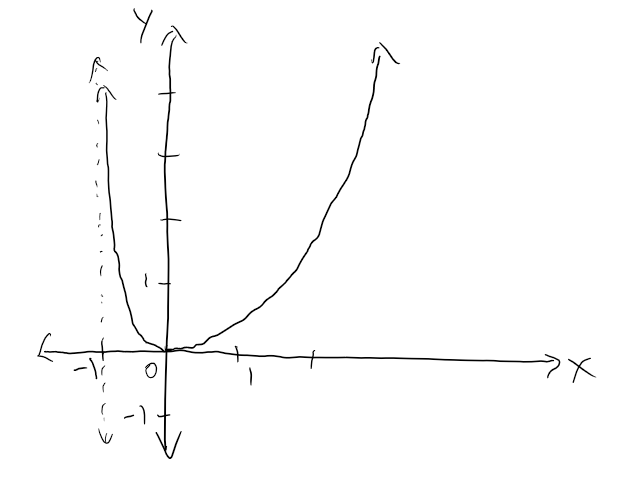
\includegraphics[width=0.5\linewidth]{q5a.png}
\end{figure}

\subproblem{b}
$f(x)=\dfrac{x^2-5x+6}{x^2-x}$
\begin{gather*}
    D_f:\{ x\in \mathbb{R} \, | \, x\ne 0,1\}\\
    \text{$y$-intercept}:(2,0),(3,0)\\
    \text{No Symmetry}\\
    \lim_{x\to -\infty}f(x)=1\\
    \lim_{x\to 0^-}f(x)=\infty\\
    \lim_{x\to 0^+}f(x)=-\infty\\
    \lim_{x\to 1^-}f(x)=-\infty\\
    \lim_{x\to 1^+}f(x)=\infty\\
    \lim_{x\to \infty}f(x)=1\\
    f'(x)=\frac{(2x-5)(x^2-x)-(2x-1)(x^2-5x+6)}{(x^2-x)^2}\\
    2x^2-6x+3=0 \implies x=\frac{3\pm\sqrt{3}}{2}\\
    f'(x)<0, \quad x\in(\frac{3-\sqrt{3}}{2}, \frac{3+\sqrt{3}}{2})\\
    f'(x)>0, \quad x\in (-\infty, \frac{3-\sqrt{3}}{2}) \cup (\frac{3+\sqrt{3}}{2},\infty)\\
    \min: f(\frac{3+\sqrt{3}}{2})\\
    \max: f(\frac{3-\sqrt{3}}{2})
\end{gather*}
\begin{figure}[H]
    \centering
    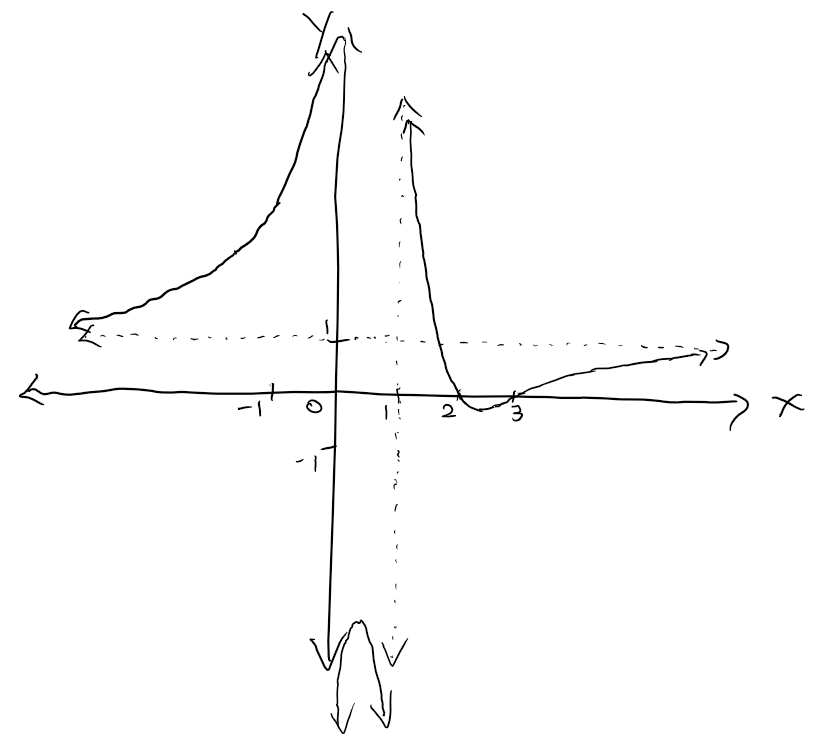
\includegraphics[width=0.5\linewidth]{q5b.png}
\end{figure}

\problem{6}
Sketch the graph of $f(x)=xe^x$ using calculus techniques. Then find:
\begin{figure}[H]
    \centering
    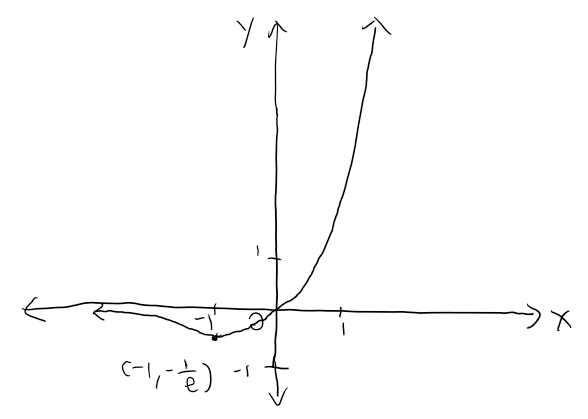
\includegraphics[width=0.5\linewidth]{q6.png}
\end{figure}

\subproblem{a}
range of $f(x)$
\begin{gather*}
    f'(x)=e^x(x+1)\\
    f'(x)=0 \implies x=-1
\end{gather*}
As $f'(x)$ changes from negative to positive at $x=-1$, $f(x)$ has a local minimum at $x=-1$. 
\begin{gather*}
    f(-1)=-\frac{1}{e}\\
    \lim_{x \to -\infty}f(x)\to 0\\
    \lim_{x \to \infty}f(x)\to \infty\\
    \boxed{f(x)\in [-\frac{1}{e},\infty)}
\end{gather*}

\subproblem{b}
point of inflection
\begin{gather*}
    f''(x)=e^x(x+2)\\
    f''(x)=0 \implies \boxed{x=-2}
\end{gather*}

\subproblem{c}
values of $k$ such that $xe^x=k$ has two distinct real roots.
\[
\boxed{k\in (-\frac{1}{e},0)}
\]

\problem{7}
Prove that there exist exactly two non-similar isosceles triangles $ABC$ such that:
\[
\tan A+\tan B +\tan C=100
\]
\begin{gather*}
    \begin{cases}
        A=B\\
        A+B+C=\pi
    \end{cases}
\end{gather*} 
\vspace{-2em}
\begin{align*}
    f(x)&=2\tan x+\tan (\pi-2x)\\
    &=2\tan x-\tan 2x\\
    &=2\tan -\frac{2\tan x}{1-\tan^2x}\\
    &=\frac{2\tan^3 x}{\tan ^2x-1}, \quad x\in (0,\frac{\pi}{2})
\end{align*}
Let $\tan x=u, \quad u\in (0,1)\cup (1,\infty)$
\begin{gather*}
    f(u)=\frac{2u^3}{u^2-1}=100\\
    u\in (0,1) \implies f(u)<0\\
    \begin{cases}
        \lim\limits_{x\to 1^+}f(u)\to \infty\\
        f(2)=\dfrac{16}{3}\\
        \lim\limits_{x\to \infty}f(u)\to\infty
    \end{cases}
\end{gather*}
By the intermediate value theorem, there exist exactly two values of $u\in(1,\infty)$ such that $f(u)=100$. Hence, exactly two non-similar isosceles triangles ABC satisfies
\[
\tan A+\tan B +\tan C=100
\]

\end{document}

